% Options for packages loaded elsewhere
\PassOptionsToPackage{unicode}{hyperref}
\PassOptionsToPackage{hyphens}{url}
\PassOptionsToPackage{dvipsnames,svgnames,x11names}{xcolor}
%
\documentclass[
  letterpaper,
  DIV=11,
  numbers=noendperiod]{scrartcl}

\usepackage{amsmath,amssymb}
\usepackage{lmodern}
\usepackage{iftex}
\ifPDFTeX
  \usepackage[T1]{fontenc}
  \usepackage[utf8]{inputenc}
  \usepackage{textcomp} % provide euro and other symbols
\else % if luatex or xetex
  \usepackage{unicode-math}
  \defaultfontfeatures{Scale=MatchLowercase}
  \defaultfontfeatures[\rmfamily]{Ligatures=TeX,Scale=1}
\fi
% Use upquote if available, for straight quotes in verbatim environments
\IfFileExists{upquote.sty}{\usepackage{upquote}}{}
\IfFileExists{microtype.sty}{% use microtype if available
  \usepackage[]{microtype}
  \UseMicrotypeSet[protrusion]{basicmath} % disable protrusion for tt fonts
}{}
\makeatletter
\@ifundefined{KOMAClassName}{% if non-KOMA class
  \IfFileExists{parskip.sty}{%
    \usepackage{parskip}
  }{% else
    \setlength{\parindent}{0pt}
    \setlength{\parskip}{6pt plus 2pt minus 1pt}}
}{% if KOMA class
  \KOMAoptions{parskip=half}}
\makeatother
\usepackage{xcolor}
\setlength{\emergencystretch}{3em} % prevent overfull lines
\setcounter{secnumdepth}{-\maxdimen} % remove section numbering
% Make \paragraph and \subparagraph free-standing
\ifx\paragraph\undefined\else
  \let\oldparagraph\paragraph
  \renewcommand{\paragraph}[1]{\oldparagraph{#1}\mbox{}}
\fi
\ifx\subparagraph\undefined\else
  \let\oldsubparagraph\subparagraph
  \renewcommand{\subparagraph}[1]{\oldsubparagraph{#1}\mbox{}}
\fi

\usepackage{color}
\usepackage{fancyvrb}
\newcommand{\VerbBar}{|}
\newcommand{\VERB}{\Verb[commandchars=\\\{\}]}
\DefineVerbatimEnvironment{Highlighting}{Verbatim}{commandchars=\\\{\}}
% Add ',fontsize=\small' for more characters per line
\usepackage{framed}
\definecolor{shadecolor}{RGB}{241,243,245}
\newenvironment{Shaded}{\begin{snugshade}}{\end{snugshade}}
\newcommand{\AlertTok}[1]{\textcolor[rgb]{0.68,0.00,0.00}{#1}}
\newcommand{\AnnotationTok}[1]{\textcolor[rgb]{0.37,0.37,0.37}{#1}}
\newcommand{\AttributeTok}[1]{\textcolor[rgb]{0.40,0.45,0.13}{#1}}
\newcommand{\BaseNTok}[1]{\textcolor[rgb]{0.68,0.00,0.00}{#1}}
\newcommand{\BuiltInTok}[1]{\textcolor[rgb]{0.00,0.23,0.31}{#1}}
\newcommand{\CharTok}[1]{\textcolor[rgb]{0.13,0.47,0.30}{#1}}
\newcommand{\CommentTok}[1]{\textcolor[rgb]{0.37,0.37,0.37}{#1}}
\newcommand{\CommentVarTok}[1]{\textcolor[rgb]{0.37,0.37,0.37}{\textit{#1}}}
\newcommand{\ConstantTok}[1]{\textcolor[rgb]{0.56,0.35,0.01}{#1}}
\newcommand{\ControlFlowTok}[1]{\textcolor[rgb]{0.00,0.23,0.31}{#1}}
\newcommand{\DataTypeTok}[1]{\textcolor[rgb]{0.68,0.00,0.00}{#1}}
\newcommand{\DecValTok}[1]{\textcolor[rgb]{0.68,0.00,0.00}{#1}}
\newcommand{\DocumentationTok}[1]{\textcolor[rgb]{0.37,0.37,0.37}{\textit{#1}}}
\newcommand{\ErrorTok}[1]{\textcolor[rgb]{0.68,0.00,0.00}{#1}}
\newcommand{\ExtensionTok}[1]{\textcolor[rgb]{0.00,0.23,0.31}{#1}}
\newcommand{\FloatTok}[1]{\textcolor[rgb]{0.68,0.00,0.00}{#1}}
\newcommand{\FunctionTok}[1]{\textcolor[rgb]{0.28,0.35,0.67}{#1}}
\newcommand{\ImportTok}[1]{\textcolor[rgb]{0.00,0.46,0.62}{#1}}
\newcommand{\InformationTok}[1]{\textcolor[rgb]{0.37,0.37,0.37}{#1}}
\newcommand{\KeywordTok}[1]{\textcolor[rgb]{0.00,0.23,0.31}{#1}}
\newcommand{\NormalTok}[1]{\textcolor[rgb]{0.00,0.23,0.31}{#1}}
\newcommand{\OperatorTok}[1]{\textcolor[rgb]{0.37,0.37,0.37}{#1}}
\newcommand{\OtherTok}[1]{\textcolor[rgb]{0.00,0.23,0.31}{#1}}
\newcommand{\PreprocessorTok}[1]{\textcolor[rgb]{0.68,0.00,0.00}{#1}}
\newcommand{\RegionMarkerTok}[1]{\textcolor[rgb]{0.00,0.23,0.31}{#1}}
\newcommand{\SpecialCharTok}[1]{\textcolor[rgb]{0.37,0.37,0.37}{#1}}
\newcommand{\SpecialStringTok}[1]{\textcolor[rgb]{0.13,0.47,0.30}{#1}}
\newcommand{\StringTok}[1]{\textcolor[rgb]{0.13,0.47,0.30}{#1}}
\newcommand{\VariableTok}[1]{\textcolor[rgb]{0.07,0.07,0.07}{#1}}
\newcommand{\VerbatimStringTok}[1]{\textcolor[rgb]{0.13,0.47,0.30}{#1}}
\newcommand{\WarningTok}[1]{\textcolor[rgb]{0.37,0.37,0.37}{\textit{#1}}}

\providecommand{\tightlist}{%
  \setlength{\itemsep}{0pt}\setlength{\parskip}{0pt}}\usepackage{longtable,booktabs,array}
\usepackage{calc} % for calculating minipage widths
% Correct order of tables after \paragraph or \subparagraph
\usepackage{etoolbox}
\makeatletter
\patchcmd\longtable{\par}{\if@noskipsec\mbox{}\fi\par}{}{}
\makeatother
% Allow footnotes in longtable head/foot
\IfFileExists{footnotehyper.sty}{\usepackage{footnotehyper}}{\usepackage{footnote}}
\makesavenoteenv{longtable}
\usepackage{graphicx}
\makeatletter
\def\maxwidth{\ifdim\Gin@nat@width>\linewidth\linewidth\else\Gin@nat@width\fi}
\def\maxheight{\ifdim\Gin@nat@height>\textheight\textheight\else\Gin@nat@height\fi}
\makeatother
% Scale images if necessary, so that they will not overflow the page
% margins by default, and it is still possible to overwrite the defaults
% using explicit options in \includegraphics[width, height, ...]{}
\setkeys{Gin}{width=\maxwidth,height=\maxheight,keepaspectratio}
% Set default figure placement to htbp
\makeatletter
\def\fps@figure{htbp}
\makeatother

\KOMAoption{captions}{tableheading}
\makeatletter
\makeatother
\makeatletter
\makeatother
\makeatletter
\@ifpackageloaded{caption}{}{\usepackage{caption}}
\AtBeginDocument{%
\ifdefined\contentsname
  \renewcommand*\contentsname{Table of contents}
\else
  \newcommand\contentsname{Table of contents}
\fi
\ifdefined\listfigurename
  \renewcommand*\listfigurename{List of Figures}
\else
  \newcommand\listfigurename{List of Figures}
\fi
\ifdefined\listtablename
  \renewcommand*\listtablename{List of Tables}
\else
  \newcommand\listtablename{List of Tables}
\fi
\ifdefined\figurename
  \renewcommand*\figurename{Figure}
\else
  \newcommand\figurename{Figure}
\fi
\ifdefined\tablename
  \renewcommand*\tablename{Table}
\else
  \newcommand\tablename{Table}
\fi
}
\@ifpackageloaded{float}{}{\usepackage{float}}
\floatstyle{ruled}
\@ifundefined{c@chapter}{\newfloat{codelisting}{h}{lop}}{\newfloat{codelisting}{h}{lop}[chapter]}
\floatname{codelisting}{Listing}
\newcommand*\listoflistings{\listof{codelisting}{List of Listings}}
\makeatother
\makeatletter
\@ifpackageloaded{caption}{}{\usepackage{caption}}
\@ifpackageloaded{subcaption}{}{\usepackage{subcaption}}
\makeatother
\makeatletter
\@ifpackageloaded{tcolorbox}{}{\usepackage[many]{tcolorbox}}
\makeatother
\makeatletter
\@ifundefined{shadecolor}{\definecolor{shadecolor}{rgb}{.97, .97, .97}}
\makeatother
\makeatletter
\makeatother
\ifLuaTeX
  \usepackage{selnolig}  % disable illegal ligatures
\fi
\IfFileExists{bookmark.sty}{\usepackage{bookmark}}{\usepackage{hyperref}}
\IfFileExists{xurl.sty}{\usepackage{xurl}}{} % add URL line breaks if available
\urlstyle{same} % disable monospaced font for URLs
\hypersetup{
  pdftitle={Baltimore Mortality Project Report},
  colorlinks=true,
  linkcolor={blue},
  filecolor={Maroon},
  citecolor={Blue},
  urlcolor={Blue},
  pdfcreator={LaTeX via pandoc}}

\title{Baltimore Mortality Project Report}
\author{}
\date{}

\begin{document}
\maketitle
\ifdefined\Shaded\renewenvironment{Shaded}{\begin{tcolorbox}[boxrule=0pt, frame hidden, interior hidden, borderline west={3pt}{0pt}{shadecolor}, enhanced, breakable, sharp corners]}{\end{tcolorbox}}\fi

\hypertarget{introduction}{%
\subsection{Introduction}\label{introduction}}

This report provides a comprehensive analysis of mortality trends in
Baltimore, focusing on how various socioeconomic factors, such as
vehicle availability, internet access, and fast food density, affect
mortality rates across different age groups. Using data from the
Baltimore Health Department, spatial maps, scatter plots, and
statistical visualizations were created to explore the correlations
between these factors and mortality over time.

\hypertarget{data-and-methods}{%
\subsection{Data and Methods}\label{data-and-methods}}

The data for this analysis was sourced from Open Baltimore - a data set
from the Baltimore City Health Department. Open Baltimore contains the
urls for JSON files containing the data we need. Neighbourhood-specific
mortality data for six different age groups (Infant, 1-14, 15-24, 25-44,
45-64, and 65-84) were collected for between 2011 and 2018. \emph{Please
note that the mortality data for ages 85+ exists, but I was not able to
download the full Open Baltimore.csv despite many attempts. Hence, we
will demonstrate with six, rather than seven, different age groups.}

We also downloaded socioeconomic data such as Percent of Households with
No Vehicle Available, Percent of Households with No Internet at Home,
and Fast Food Outlet Density per 1,000 Residents.

In order to reproduce this analysis, we require the following libraries:

\begin{Shaded}
\begin{Highlighting}[]
\CommentTok{\# Load libraries}
\FunctionTok{library}\NormalTok{(tidyverse)}
\FunctionTok{library}\NormalTok{(jsonlite)}
\FunctionTok{library}\NormalTok{(dplyr)}
\FunctionTok{library}\NormalTok{(ggplot2)}
\FunctionTok{library}\NormalTok{(purrr)}
\FunctionTok{library}\NormalTok{(sf)}
\FunctionTok{library}\NormalTok{(knitr)}
\NormalTok{path }\OtherTok{=}\NormalTok{ here}\SpecialCharTok{::}\FunctionTok{here}\NormalTok{()}
\end{Highlighting}
\end{Shaded}

Next, we load the JSON files that were retrieved from the urls in Open
Baltimore (please see download\_data.R for detailed downloading steps).
After loading the data, we extract important features, such as mortality
rate and transform the data to long format for visualization. An example
of how this is done is below.

\begin{Shaded}
\begin{Highlighting}[]
\CommentTok{\# Function to extract attributes from the JSON structure}
\NormalTok{extract\_attributes }\OtherTok{\textless{}{-}} \ControlFlowTok{function}\NormalTok{(json\_data) \{}
  \FunctionTok{map\_df}\NormalTok{(json\_data}\SpecialCharTok{$}\NormalTok{features, }\SpecialCharTok{\textasciitilde{}}\NormalTok{ .x}\SpecialCharTok{$}\NormalTok{attributes)}
\NormalTok{\}}

\CommentTok{\# Read mortality data for each age group; here we demonstrate with the 1{-}14 group}
\NormalTok{mortality\_1\_14 }\OtherTok{\textless{}{-}} \FunctionTok{read\_json}\NormalTok{(}\FunctionTok{paste0}\NormalTok{(path, }\StringTok{"/data/json/mortality\_1{-}14.json"}\NormalTok{)) }\SpecialCharTok{\%\textgreater{}\%}
  \FunctionTok{extract\_attributes}\NormalTok{()}

\CommentTok{\# Function to reshape data to long format for plotting}
\NormalTok{reshape\_to\_long }\OtherTok{=} \ControlFlowTok{function}\NormalTok{(data, age\_group, prefix, value) \{}
\NormalTok{  data }\SpecialCharTok{\%\textgreater{}\%}
    \FunctionTok{select}\NormalTok{(CSA2010, }\FunctionTok{starts\_with}\NormalTok{(prefix)) }\SpecialCharTok{\%\textgreater{}\%}
    \FunctionTok{pivot\_longer}\NormalTok{(}\AttributeTok{cols =} \FunctionTok{starts\_with}\NormalTok{(prefix), }\AttributeTok{names\_to =} \StringTok{"year"}\NormalTok{, }
                 \AttributeTok{values\_to =} \FunctionTok{paste0}\NormalTok{(value, }\StringTok{"\_rate"}\NormalTok{)) }\SpecialCharTok{\%\textgreater{}\%}
    \FunctionTok{mutate}\NormalTok{(}\AttributeTok{year =} \FunctionTok{as.integer}\NormalTok{(}\FunctionTok{str\_extract}\NormalTok{(year, }\StringTok{"}\SpecialCharTok{\textbackslash{}\textbackslash{}}\StringTok{d+$"}\NormalTok{)),}
           \AttributeTok{age\_group =}\NormalTok{ age\_group)}
  \CommentTok{\# data$mean = rep(mean(data$morality\_rate), nrow(data))}
\NormalTok{\}}

\CommentTok{\# Reshape data}
\FunctionTok{reshape\_to\_long}\NormalTok{(mortality\_1\_14, }\StringTok{"1{-}14"}\NormalTok{, }\StringTok{"mort14"}\NormalTok{, }\StringTok{"mort"}\NormalTok{)}

\CommentTok{\# Our final data set containing all of the long{-}formatted data }
\CommentTok{\# is called mortality\_data}
\end{Highlighting}
\end{Shaded}

\hypertarget{data-visualization}{%
\subsubsection{Data visualization}\label{data-visualization}}

We used a variety of plots to visualize the relationships between
socioeconomic covariates and mortality rates over time and across age
groups. Scatter plots and trend lines were used to show correlations,
and spatial maps were generated to highlight geographical variations in
mortality.

\hypertarget{results}{%
\subsection{Results}\label{results}}

\hypertarget{mortality-trends-over-time}{%
\subsubsection{Mortality Trends Over
Time}\label{mortality-trends-over-time}}

Figure~\ref{fig-1} visualizes mortality rates across multiple age groups
(Infant, 1-14, 15-24, 25-44, 45-64, and 65-84) from 2011 to 2018.

We notice that\ldots{}

\begin{itemize}
\item
  Infant Mortality: While lower than the older age groups, there are
  notable spikes in infant mortality, particularly in 2016.
\item
  Youth (1-14 and 15-24): These groups maintain relatively low mortality
  rates over time.
\item
  Older Age Groups (45-64 and 65-84): These groups consistently exhibit
  higher mortality rates compared to younger groups. The mortality rate
  in these groups shows some fluctuations, but overall, the trend
  remains stable over time.
\end{itemize}

\begin{figure}

{\centering 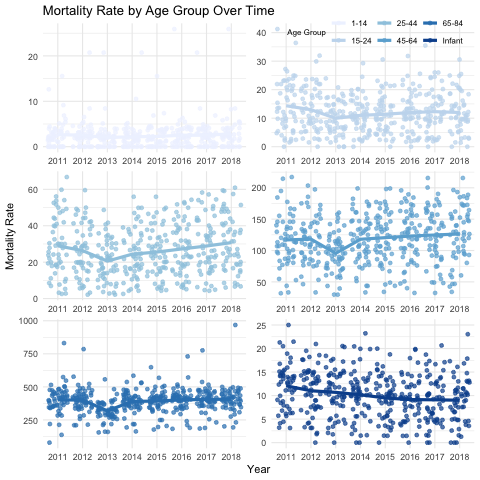
\includegraphics[width=0.65\textwidth,height=\textheight]{figures/mortality_over_time_by_age_group.png}

}

\caption{\label{fig-1}Mortality Over Time by Age Group}

\end{figure}

\hypertarget{socioeconomic-covariates-vs.-mortality-rates}{%
\subsubsection{Socioeconomic Covariates vs.~Mortality
Rates}\label{socioeconomic-covariates-vs.-mortality-rates}}

Figure~\ref{fig-2} shows the distributions of each socioeconomic
covariate across Baltimore neighbourhoods.

\begin{itemize}
\item
  Fast Food Outlet Density: The distribution is heavily skewed towards
  low fast food density per 1,000 residents with a few outliers.
\item
  Percentage of Households with No Internet at Home: A notable
  proportion of households have no internet access, with the
  distribution showing multiple peaks around 15-20\% and 25-35\%.
\item
  Percentage of Households with No Vehicles Availabile: A notable
  percentage of households lack vehicle access, with the median falling
  around 30\% and some areas reaching over 60\%.
\end{itemize}

\begin{Shaded}
\begin{Highlighting}[]
\CommentTok{\# Adding covariates (fast food data) to mortality data frame}
\NormalTok{fastfd\_data }\OtherTok{=} \FunctionTok{reshape\_to\_long}\NormalTok{(fast\_food[,}\DecValTok{1}\SpecialCharTok{:}\DecValTok{5}\NormalTok{], }\StringTok{""}\NormalTok{, }\StringTok{"Fastfd"}\NormalTok{, }\StringTok{"fastfd"}\NormalTok{) }\SpecialCharTok{\%\textgreater{}\%} 
  \FunctionTok{subset}\NormalTok{(}\AttributeTok{select =} \SpecialCharTok{{-}}\FunctionTok{c}\NormalTok{(age\_group))}
\NormalTok{fastfd\_data}\SpecialCharTok{$}\NormalTok{year }\OtherTok{=}\NormalTok{ fastfd\_data}\SpecialCharTok{$}\NormalTok{year }\SpecialCharTok{+} \DecValTok{2000}
\NormalTok{fastfd\_mortality\_data }\OtherTok{=} \FunctionTok{inner\_join}\NormalTok{(mortality\_data, fastfd\_data, }
                                   \AttributeTok{by =} \FunctionTok{c}\NormalTok{(}\StringTok{"CSA2010"}\NormalTok{, }\StringTok{"year"}\NormalTok{))}

\CommentTok{\# Plot distribution of covariates}
\FunctionTok{ggplot}\NormalTok{(fastfd\_data, }\FunctionTok{aes}\NormalTok{(}\AttributeTok{x =}\NormalTok{ fastfd\_rate)) }\SpecialCharTok{+}
  \FunctionTok{geom\_histogram}\NormalTok{(}\FunctionTok{aes}\NormalTok{(}\AttributeTok{y=}\NormalTok{..density..), }\AttributeTok{bins =} \DecValTok{50}\NormalTok{, }\AttributeTok{alpha =} \FloatTok{0.5}\NormalTok{, }\AttributeTok{fill =} \StringTok{"blue"}\NormalTok{) }\SpecialCharTok{+}
  \FunctionTok{theme\_minimal}\NormalTok{() }\SpecialCharTok{+}
  \FunctionTok{labs}\NormalTok{(}\AttributeTok{title =} \StringTok{"Distribution of Fast Food Outlet Density per 1,000 Residents"}\NormalTok{,}
       \AttributeTok{x =} \StringTok{"Fast Food Outlet Density per 1,000 Residents"}\NormalTok{,}
       \AttributeTok{y =} \StringTok{"Frequency"}\NormalTok{) }
\end{Highlighting}
\end{Shaded}

\begin{figure}

{\centering 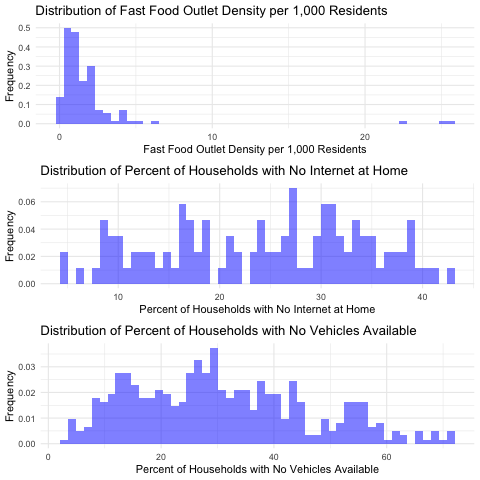
\includegraphics[width=0.65\textwidth,height=\textheight]{figures/distribution_of_covariates.png}

}

\caption{\label{fig-2}Distribution of Socioeconomic Covariates}

\end{figure}

\begin{Shaded}
\begin{Highlighting}[]
\CommentTok{\# Relationship between Fast Food Density and Mortality }
\FunctionTok{ggplot}\NormalTok{(fastfd\_mortality\_data, }\FunctionTok{aes}\NormalTok{(}\AttributeTok{x =}\NormalTok{ mort\_rate, }\AttributeTok{y =}\NormalTok{ fastfd\_rate, }\AttributeTok{color =} \FunctionTok{as.factor}\NormalTok{(year))) }\SpecialCharTok{+}
  \FunctionTok{geom\_jitter}\NormalTok{(}\AttributeTok{alpha =} \FloatTok{0.7}\NormalTok{) }\SpecialCharTok{+}
  \FunctionTok{geom\_smooth}\NormalTok{() }\SpecialCharTok{+}
 \FunctionTok{facet\_wrap}\NormalTok{(}\SpecialCharTok{\textasciitilde{}}\NormalTok{year, }\AttributeTok{scales =} \StringTok{"free"}\NormalTok{, }\AttributeTok{ncol =} \DecValTok{2}\NormalTok{) }\SpecialCharTok{+}
  \FunctionTok{theme\_minimal}\NormalTok{() }\SpecialCharTok{+}
  \FunctionTok{labs}\NormalTok{(}\AttributeTok{title =} \StringTok{"Fast Food Density vs. Mortality Rate Over Time by Year"}\NormalTok{,}
       \AttributeTok{x =} \StringTok{"Mortality Rate"}\NormalTok{,}
       \AttributeTok{y =} \StringTok{"Fast Food Outlet Density per 1,000 Residents"}\NormalTok{) }\SpecialCharTok{+}
  \FunctionTok{scale\_color\_brewer}\NormalTok{(}\StringTok{"Year"}\NormalTok{, }\AttributeTok{palette =} \StringTok{"Blues"}\NormalTok{) }\SpecialCharTok{+}
  \FunctionTok{theme}\NormalTok{(}\AttributeTok{legend.position =} \StringTok{"bottom"}\NormalTok{, }
        \AttributeTok{legend.direction =}\StringTok{"horizontal"}\NormalTok{,}
        \AttributeTok{legend.text =} \FunctionTok{element\_text}\NormalTok{(}\AttributeTok{size =} \DecValTok{8}\NormalTok{),}
        \AttributeTok{legend.title =} \FunctionTok{element\_text}\NormalTok{(}\AttributeTok{size =} \DecValTok{8}\NormalTok{),}
        \AttributeTok{plot.title =} \FunctionTok{element\_text}\NormalTok{(}\AttributeTok{size =} \DecValTok{14}\NormalTok{)) }

\CommentTok{\# Relationship between Fast Food Density and Mortality }
\FunctionTok{ggplot}\NormalTok{(fastfd\_mortality\_data, }\FunctionTok{aes}\NormalTok{(}\AttributeTok{x =}\NormalTok{ mort\_rate, }\AttributeTok{y =}\NormalTok{ fastfd\_rate, }\AttributeTok{color =} \FunctionTok{as.factor}\NormalTok{(year))) }\SpecialCharTok{+}
  \FunctionTok{geom\_jitter}\NormalTok{(}\AttributeTok{alpha =} \FloatTok{0.7}\NormalTok{) }\SpecialCharTok{+}
  \FunctionTok{geom\_smooth}\NormalTok{() }\SpecialCharTok{+}
 \FunctionTok{facet\_wrap}\NormalTok{(}\SpecialCharTok{\textasciitilde{}}\NormalTok{age\_group, }\AttributeTok{scales =} \StringTok{"free"}\NormalTok{, }\AttributeTok{ncol =} \DecValTok{2}\NormalTok{) }\SpecialCharTok{+}
  \FunctionTok{theme\_minimal}\NormalTok{() }\SpecialCharTok{+}
  \FunctionTok{labs}\NormalTok{(}\AttributeTok{title =} \StringTok{"Fast Food Density vs. Mortality Rate by Age Group"}\NormalTok{,}
       \AttributeTok{x =} \StringTok{"Mortality Rate"}\NormalTok{,}
       \AttributeTok{y =} \StringTok{"Fast Food Outlet Density per 1,000 Residents"}\NormalTok{) }\SpecialCharTok{+}
  \FunctionTok{scale\_color\_brewer}\NormalTok{(}\StringTok{"Year"}\NormalTok{, }\AttributeTok{palette =} \StringTok{"Blues"}\NormalTok{) }\SpecialCharTok{+}
  \FunctionTok{theme}\NormalTok{(}\AttributeTok{legend.position =} \StringTok{"bottom"}\NormalTok{, }
        \AttributeTok{legend.direction =}\StringTok{"horizontal"}\NormalTok{,}
        \AttributeTok{legend.text =} \FunctionTok{element\_text}\NormalTok{(}\AttributeTok{size =} \DecValTok{8}\NormalTok{),}
        \AttributeTok{legend.title =} \FunctionTok{element\_text}\NormalTok{(}\AttributeTok{size =} \DecValTok{8}\NormalTok{),}
        \AttributeTok{plot.title =} \FunctionTok{element\_text}\NormalTok{(}\AttributeTok{size =} \DecValTok{14}\NormalTok{)) }
\end{Highlighting}
\end{Shaded}

Figure~\ref{fig-3} through Figure~\ref{fig-8} illustrate the
relationships between each of the socioeconomic covariates and mortality
rates, stratified by year and by age group. For each covariate, we
isolated the data to years where mortality data was also reported.
First, we show the distributions of each covariate.

\hypertarget{fast-food-outlet-density-and-mortality-rate-correlation}{%
\paragraph{Fast Food Outlet Density and Mortality Rate
Correlation}\label{fast-food-outlet-density-and-mortality-rate-correlation}}

\begin{itemize}
\item
  The smoothed line in Figure~\ref{fig-3} suggests that fast food
  density correlates positively with higher mortality rates, especially
  in the later years of the dataset. However, it is important to note
  that these results are greatly affected by a few extreme points.
  Therefore, we cannot make any conclusions about any associations.
\item
  Figure~\ref{fig-4} shows the age group trends. Although fast food
  availability may be linked to poorer health outcomes in theory, these
  trends are not present in our data. The absence of clear trends and
  the presence of some extreme outliers prevent us from making any
  conclusions.
\end{itemize}

\begin{figure}

{\centering 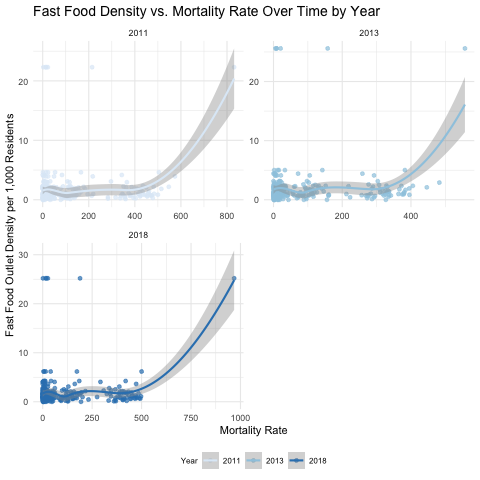
\includegraphics[width=0.65\textwidth,height=\textheight]{figures/fastfd_vs_mortality_by_year.png}

}

\caption{\label{fig-3}Fast Food vs.~Mortality Rate by Year}

\end{figure}

\begin{figure}

{\centering 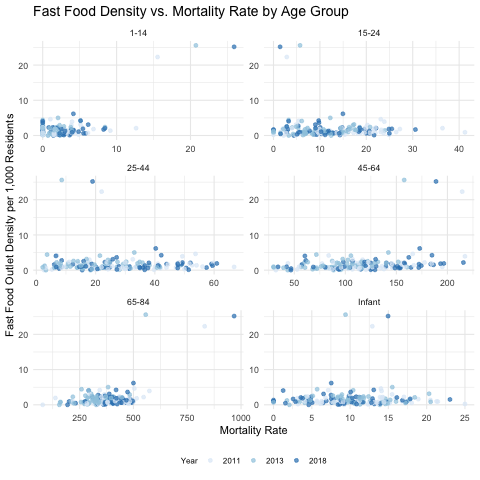
\includegraphics[width=0.65\textwidth,height=\textheight]{figures/fastfd_vs_mortality_by_age.png}

}

\caption{\label{fig-4}Fast Food vs.~Mortality Rate by Age Group}

\end{figure}

\hypertarget{home-internet-access-and-mortality-rate-correlation}{%
\paragraph{Home Internet Access and Mortality Rate
Correlation}\label{home-internet-access-and-mortality-rate-correlation}}

\begin{itemize}
\item
  As shown in Figure~\ref{fig-5}, we only have internet data for 2017
  and 2018. There is no dicernable trend when we stratify by year.
  However, we notice that the data points can be split into sections,
  which suggest there may be age group trends.
\item
  Figure~\ref{fig-6} shows a clear positive trend between mortality rate
  and lack of home internet access, in particular for ages 15-64. The
  trend is less pronounced in Infant, 1-14, and 65-84 age groups.
\end{itemize}

\begin{figure}

{\centering 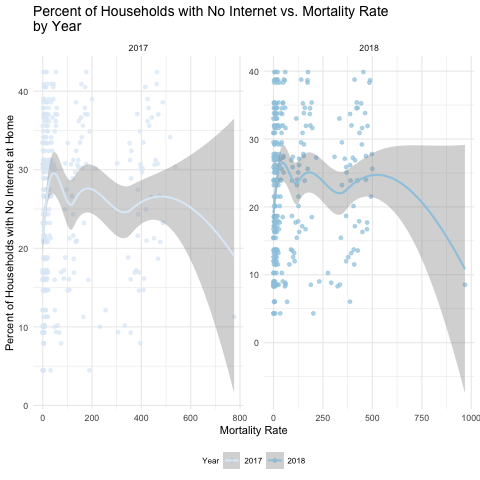
\includegraphics[width=0.65\textwidth,height=\textheight]{figures/nohhint_vs_mortality_by_year.png}

}

\caption{\label{fig-5}Home Internet Access vs.~Mortality Rate by Year}

\end{figure}

\begin{figure}

{\centering 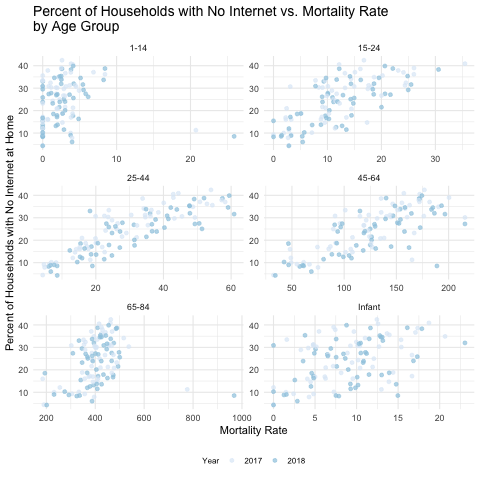
\includegraphics[width=0.65\textwidth,height=\textheight]{figures/nohhint_vs_mortality_by_age.png}

}

\caption{\label{fig-6}Home Internet Access vs.~Mortality Rate by Age
Group}

\end{figure}

\hypertarget{vehicle-access-and-mortality-rate-correlation}{%
\paragraph{Vehicle Access and Mortality Rate
Correlation}\label{vehicle-access-and-mortality-rate-correlation}}

\begin{itemize}
\item
  Figure~\ref{fig-7} shows that from 2011 to 2018, there seems to be
  groups of data points that have a positive correlation between the
  percentage of households without vehicle access and higher mortality
  rates. This suggests a multilevel structure to the data, and perhaps
  we should stratefy it by age group.
\item
  Figure~\ref{fig-8} shows that there is indeed a positive correlation
  between lower rates of vehicle availability and higher rates of
  mortality Again, the trend is less pronounced in Infant, 1-14, and
  65-84 age groups.
\end{itemize}

\begin{figure}

{\centering 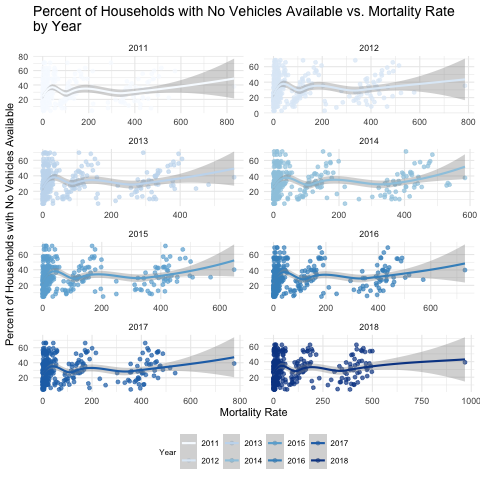
\includegraphics[width=0.65\textwidth,height=\textheight]{figures/novhcl_vs_mortality_by_year.png}

}

\caption{\label{fig-7}Vehicle Availability vs.~Mortality Rate by Year}

\end{figure}

\begin{figure}

{\centering 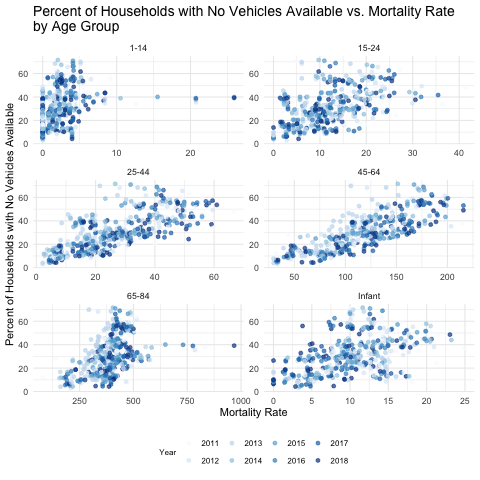
\includegraphics[width=0.65\textwidth,height=\textheight]{figures/novhcl_vs_mortality_by_age.png}

}

\caption{\label{fig-8}Vehicle Availability vs.~Mortality Rate by Age
Group}

\end{figure}

\hypertarget{spatial-distribution-of-mortality-rates-by-year-and-age-group}{%
\subsubsection{Spatial Distribution of Mortality Rates by Year and Age
Group}\label{spatial-distribution-of-mortality-rates-by-year-and-age-group}}

Figure~\ref{fig-9} presents spatial maps of mortality rates across
Baltimore from 2011 to 2018 for different age groups. Each row
corresponds to an age group, and each column to a year.

\begin{itemize}
\item
  Geographical Mortality Patterns: Hotspots for mortality consistently
  appear in certain areas of Baltimore. For example, areas in the
  northern and central regions exhibit high mortality rates across
  different age groups. Infant mortality appears to be much higher in a
  few central regions than in surrounding regions.
\item
  Temporal Changes: While certain hotspots remain constant, there are
  areas where mortality fluctuates. Some hotspots, particularly in the
  infant and 15-24 age groups, appear to have decreasing mortality rates
  over time. Other hotspots in the 65-84 group, for example, seem to
  have increasing mortality rates in more recent years.
\end{itemize}

\begin{Shaded}
\begin{Highlighting}[]
\CommentTok{\# Read in the JSON data for mortality\_infant}
\NormalTok{res }\OtherTok{\textless{}{-}} \FunctionTok{read\_json}\NormalTok{(}\FunctionTok{paste0}\NormalTok{(path, }\StringTok{"/data/json/mortality\_1{-}14.json"}\NormalTok{), }\AttributeTok{simplifyVector =} \ConstantTok{FALSE}\NormalTok{)}
\NormalTok{df }\OtherTok{\textless{}{-}}\NormalTok{ purrr}\SpecialCharTok{::}\FunctionTok{map}\NormalTok{(res}\SpecialCharTok{$}\NormalTok{features, }\ControlFlowTok{function}\NormalTok{(r) \{}
    \ControlFlowTok{if}\NormalTok{ (}\SpecialCharTok{!}\FunctionTok{is.null}\NormalTok{(r}\SpecialCharTok{$}\NormalTok{geometry) }\SpecialCharTok{\&\&} \SpecialCharTok{!}\FunctionTok{is.null}\NormalTok{(r}\SpecialCharTok{$}\NormalTok{geometry}\SpecialCharTok{$}\NormalTok{rings) }\SpecialCharTok{\&\&} \FunctionTok{length}\NormalTok{(r}\SpecialCharTok{$}\NormalTok{geometry}\SpecialCharTok{$}\NormalTok{rings) }\SpecialCharTok{\textgreater{}} \DecValTok{0}\NormalTok{) \{}
      \CommentTok{\# Loop over each ring layer and extract coordinates}
\NormalTok{      rings\_data }\OtherTok{\textless{}{-}}\NormalTok{ purrr}\SpecialCharTok{::}\FunctionTok{map}\NormalTok{(r}\SpecialCharTok{$}\NormalTok{geometry}\SpecialCharTok{$}\NormalTok{rings, }\ControlFlowTok{function}\NormalTok{(ring) \{}
        \FunctionTok{do.call}\NormalTok{(rbind, purrr}\SpecialCharTok{::}\FunctionTok{map}\NormalTok{(ring, unlist)) }\SpecialCharTok{\%\textgreater{}\%}
          \FunctionTok{as.data.frame}\NormalTok{(}\AttributeTok{stringsAsFactors =} \ConstantTok{FALSE}\NormalTok{)}
\NormalTok{      \})}
      \CommentTok{\# Combine the multiple rings into a single data frame}
\NormalTok{      x }\OtherTok{\textless{}{-}} \FunctionTok{bind\_rows}\NormalTok{(rings\_data)}
      \FunctionTok{colnames}\NormalTok{(x) }\OtherTok{\textless{}{-}} \FunctionTok{c}\NormalTok{(}\StringTok{"lon"}\NormalTok{, }\StringTok{"lat"}\NormalTok{)}
\NormalTok{      x}\SpecialCharTok{$}\NormalTok{CSA2010 }\OtherTok{\textless{}{-}}\NormalTok{ r}\SpecialCharTok{$}\NormalTok{attributes}\SpecialCharTok{$}\NormalTok{CSA2010 }\CommentTok{\# Include CSA2010}
      \FunctionTok{return}\NormalTok{(x)}
\NormalTok{    \} }\ControlFlowTok{else}\NormalTok{ \{}
      \FunctionTok{return}\NormalTok{(}\ConstantTok{NULL}\NormalTok{)}
\NormalTok{    \}}
\NormalTok{  \})}
\NormalTok{out }\OtherTok{\textless{}{-}}\NormalTok{ res }\SpecialCharTok{\%\textgreater{}\%} \FunctionTok{extract\_attributes}\NormalTok{()}
\FunctionTok{names}\NormalTok{(df) }\OtherTok{=}\NormalTok{ out}\SpecialCharTok{$}\NormalTok{CSA2010}
\NormalTok{df }\OtherTok{=}\NormalTok{ dplyr}\SpecialCharTok{::}\FunctionTok{bind\_rows}\NormalTok{(df, }\AttributeTok{.id =} \StringTok{"CSA2010"}\NormalTok{)}
\NormalTok{polygon }\OtherTok{\textless{}{-}}\NormalTok{ df }\SpecialCharTok{\%\textgreater{}\%}
  \FunctionTok{group\_by}\NormalTok{(CSA2010) }\SpecialCharTok{\%\textgreater{}\%}
  \FunctionTok{st\_as\_sf}\NormalTok{(}\AttributeTok{coords =} \FunctionTok{c}\NormalTok{(}\StringTok{"lon"}\NormalTok{, }\StringTok{"lat"}\NormalTok{), }\AttributeTok{crs =} \DecValTok{4326}\NormalTok{) }\SpecialCharTok{\%\textgreater{}\%}
  \FunctionTok{summarise}\NormalTok{(}\AttributeTok{geometry =} \FunctionTok{st\_combine}\NormalTok{(geometry)) }\SpecialCharTok{\%\textgreater{}\%}
  \FunctionTok{st\_cast}\NormalTok{(}\StringTok{"POLYGON"}\NormalTok{) }\SpecialCharTok{\%\textgreater{}\%}
  \FunctionTok{left\_join}\NormalTok{(mortality\_data, }\AttributeTok{by =} \StringTok{"CSA2010"}\NormalTok{)}

\NormalTok{P1 }\OtherTok{=} \FunctionTok{ggplot}\NormalTok{() }\SpecialCharTok{+}
  \FunctionTok{geom\_sf}\NormalTok{(}\AttributeTok{data =} \FunctionTok{filter}\NormalTok{(polygon, age\_group }\SpecialCharTok{==} \StringTok{"Infant"}\NormalTok{), }\FunctionTok{aes}\NormalTok{(}\AttributeTok{fill =}\NormalTok{ mort\_rate)) }\SpecialCharTok{+}
  \FunctionTok{facet\_wrap}\NormalTok{( }\SpecialCharTok{\textasciitilde{}}\NormalTok{ year, }\AttributeTok{ncol =} \DecValTok{8}\NormalTok{) }\SpecialCharTok{+} 
  \FunctionTok{labs}\NormalTok{(}\AttributeTok{x =} \StringTok{""}\NormalTok{, }\AttributeTok{y =} \StringTok{""}\NormalTok{) }\SpecialCharTok{+}
  \FunctionTok{scale\_y\_continuous}\NormalTok{() }\SpecialCharTok{+}
  \FunctionTok{scale\_fill\_viridis\_c}\NormalTok{(}\StringTok{"Mortality }\SpecialCharTok{\textbackslash{}n}\StringTok{Rate"}\NormalTok{, }\AttributeTok{option =} \StringTok{"C"}\NormalTok{, }\AttributeTok{na.value =} \StringTok{"grey50"}\NormalTok{) }\SpecialCharTok{+}
  \CommentTok{\#scale\_fill\_distiller("Mortality Rate", palette = "Blues") + }
  \FunctionTok{theme\_minimal}\NormalTok{() }\SpecialCharTok{+} \CommentTok{\# Clean theme}
  \FunctionTok{theme}\NormalTok{(}
    \AttributeTok{axis.text.x =} \FunctionTok{element\_blank}\NormalTok{(), }\CommentTok{\# Remove y{-}axis labels}
    \AttributeTok{axis.text.y =} \FunctionTok{element\_blank}\NormalTok{(), }\CommentTok{\# Remove y{-}axis labels}
    \AttributeTok{strip.text =} \FunctionTok{element\_text}\NormalTok{(}\AttributeTok{size =} \DecValTok{16}\NormalTok{),}\CommentTok{\# Adjust facet label size}
    \AttributeTok{legend.title =} \FunctionTok{element\_text}\NormalTok{(}\AttributeTok{size =} \DecValTok{12}\NormalTok{),}
    \AttributeTok{legend.key.size =} \FunctionTok{unit}\NormalTok{(}\DecValTok{10}\NormalTok{, }\StringTok{"mm"}\NormalTok{),}
    \AttributeTok{legend.position =} \StringTok{"right"}
\NormalTok{  )}
\NormalTok{P1\_labeled }\OtherTok{\textless{}{-}} \FunctionTok{add\_labels}\NormalTok{(P1, }\AttributeTok{left\_label =} \StringTok{"Infant"}\NormalTok{)}
\end{Highlighting}
\end{Shaded}

\begin{figure}

{\centering \includegraphics[width=15in,height=\textheight]{figures/mortality_maps.png}

}

\caption{\label{fig-9}Baltimore Mortality Map}

\end{figure}

\hypertarget{discussion}{%
\subsection{Discussion}\label{discussion}}

The findings highlight significant spatial, temporal, and socioeconomic
disparities in mortality rates across Baltimore. Key correlations
emerged between mortality and the availability of vehicles, internet
access, and fast food density, particularly among older age groups.

The socioeconomic associations with mortality rates can motivate
important public health considerations. Although fast food density
appears to have little association with mortality rate, there are clear
associations between lower rates of home internet access and vehicle
availability with higher mortality rate. The trend is less clear in
infant and 1-14 age groups, potentially because these populations are
less likely to rely on internet and vehicles in their daily life.
Furthermore, these populations have very low mortality rates. Primary
drivers of youth mortality may be due to issues other than the
socioeconomic covariates we tested. Furthermore, in the 65-84
population, the associations are also less apparent. This can be, in
part, explained by the fact that health conditions related to old age
may have a stronger impact on mortality rates than socioeconomic
conditions.

Some limitations of the study include that this analysis relies on
correlation data and cannot make causal inferences. Further research
should explore causal pathways and investigate additional socioeconomic
factors that may contribute to the observed disparities in mortality.

This analysis highlights the complex interplay between socioeconomic
factors and mortality rates across Baltimore. By focusing on both
geographic and temporal trends, we have identified critical areas where
public health interventions may be most effective in reducing mortality
rates and addressing health disparities.



\end{document}
